\subsection{\texttt{Physics} project}
The Physics component is responsible for collision detection, ray casting, and physical modeling.
The main purpose of this component is to expose the various functionalities of the BepuPhysics2 library to the rest of the system.
The component also makes extensive use of the code from the BepuPhysics2 Demos project.

Each game object is represented by a \textit{body} (each body has an associated \textit{body handle}) in the physics engine.
This one-to-one mapping is stored in the \texttt{Scene} class in an object of \texttt{SimulationMembers} type.
\texttt{SimulationMembers} allows for adding and removing simulation members as well as accessing handles to bodies in the physics engine associated with a given game object.
Game objects are represented by either simple or composite shapes in the physical simulation.
Simple shapes used in the game include cylinders, capsules, and boxes.
Composite shapes arise by composing simple shapes.
\question{Should the car be described in more detail (how to specify the axis of rotation for the wheels, etc.)}

To facilitate debugging, the Physics component also provides a way to extract all shapes from the simulation (and decompose composite shapes) which then can be shown in debug mode, see \autoref{fig:bounding-shapes}.
When shown, the bounding shapes can be either green or red depending on whether the corresponding bodies are in the active or inactive state in the physics engine.
In \autoref{fig:bounding-shapes} it can be seen that the player has been hit by a projectile which caused the player's body to become active (or \textit{awakend} using the BepuPhysics parlance) as indicated by the green bounding shape.
The projectile that hit the player can also be seen to be active.
On the other hand, the projectiles that fell to the ground and had been still for some time became inactive as marked by the red bounding shapes.
\begin{figure}[h]
    \centering
    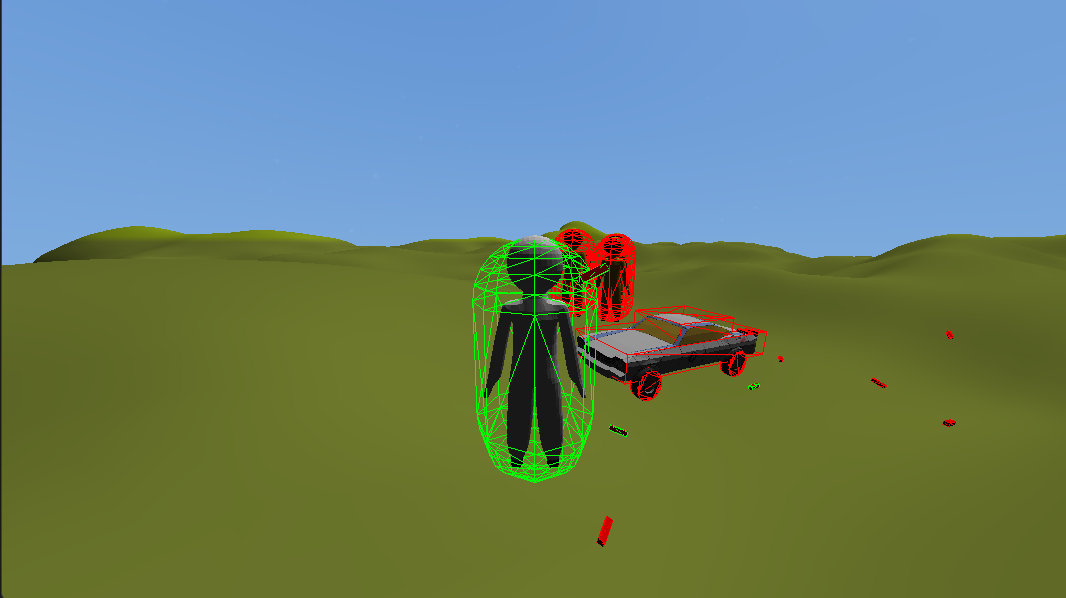
\includegraphics[width=0.8\textwidth]{chapters/implementation/sections/game_objects_management/subsections/physics_project/resources/bounding-shapes.png}
    \caption{Game objects enclosed in bounding shapes for collision detection}
    \label{fig:bounding-shapes}
\end{figure}

The body that represents the terrain was created as a separate shape from the terrain mesh triangle-by-triangle.

Game objects can listen and respond to collisions by registering their contact callbacks via the API in \texttt{SimulationManager}.
Such objects implement the \texttt{IContactEventListener} interface whose implementations define the contact callbacks.
The only information about the collision is which two bodies collided and where.

Some game objects can cast rays.
An example of such an object is the player who uses a ray to define a place where terrain modification should take place.
Each ray in the physics engine has an ID number, direction, etc.
An object that wishes to cast rays has to therefore implement an interface (\texttt{IRayCaster}) that exposes all the necessary information.